\section{CPV in Kaon System} 
\vspace{-1.0em}
\begin{center}
\tiny{\textit{Kevin Maguire}}
\end{center}

\subsection{Neutral Kaon Mixing}

As mentioned CPV was first observed in the neutral Kaon system. Direct and indirect CPV have been observed but it is found that the process is entirely dominated by the indirect method. Essential to these mechanisms is the mixing between the neutral Kaon and its anti-particle, corresponding to the states $\ket{K^{0}}$ and $\ket{\bar{K}^{0}}$. These have quark compositions of $d \bar{s}$ and $s \bar{d}$, respectively. 

In interactions involving the strong or EM force, the quantum number strangeness, which tells us the number of strange quarks in a particle, must be conserved. For the weak force it is found that, like parity, this symmetry is not conserved. Due to this many processes forbidden for the strong and EM interactions are allowed through the weak force. This violation is what makes mixing possible. Mixing is the decay of a particle into its anti-particle and can only take place when a particle is its own anti-particle, or if the particles differ by a quantum number which is not conserved by some interaction. This is the case in neutral Kaon mixing, also know as Kaon oscillations. The neutral Kaon and its anti-particle have opposite strangeness but can decay into each other through the strangeness violating weak force. See \cref{KaonMixinFeyn}. 

\begin{figure}[h!]
\begin{center}
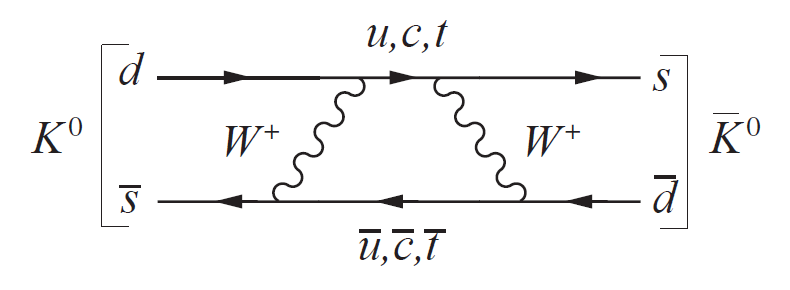
\includegraphics[scale=0.4]{figs/KevFeyn1.png}
\end{center}
\caption{\textit{Feynmann diagram illustrating the process through which neutral Kaons decay into eachother}}
\label{KaonMixinFeyn}
\end{figure}

Analogous to the mixing of mass eigenstate quarks to different quark flavours, it is found that the neutral Kaon flavour eigenstates do not correspond to eigenstates of the $\hat{C}\hat{P}$ operator. To show this first operate on the Kaon states with $\hat{C}$. Neglecting phase throughout and assuming no CPV for now, one obtains:

\begin{align*}
\hat{C} \ket{K^{0}(d \bar{s})} = (1)(-1) \ket{\bar{K}^{0}(s \bar{d})} = - \ket{\bar{K}^{0}(s \bar{d})}  \\
\hat{C} \ket{\bar{K}^{0}(s \bar{d})} = (1)(-1) \ket{K^{0}(d \bar{s})} = - \ket{K^{0}(d \bar{s})}  
\end{align*}

\noindent Where we have used the convention that $C (q) = 1$ and ${C} (\bar{q}) = -1$. Also, the action of the $\hat{P}$ operator is given by:
    
\begin{align*}
\hat{P} \ket{K^{0}(d \bar{s})} = {P}(d) {P}(\bar{s})(-1)^{l} \ket{K^{0}(d \bar{s})} = (1)(-1)(-1)^0 \ket{K^{0}(d \bar{s})} = - \ket{K^{0}(d \bar{s})} \\
\hat{P} \ket{\bar{K}^{0}(s \bar{d})} = {P}(s) {P}(\bar{d})(-1)^{l} \ket{\bar{K}^{0}(s \bar{d})} = (1)(-1)(-1)^0 \ket{\bar{K}^{0}(s \bar{d})} = - \ket{\bar{K}^{0}(s \bar{d})} 
\end{align*}

\smallskip

\noindent Where we have used the convention ${P} (fermion) = 1$ and ${P} (anti-fermion) = -1$ as well as $l=0$ because the Kaon is the lowest energy combination of these quarks and itself has a $J^{P}$ of $0^{-}$. Now the eigenstates of $\hat{C}\hat{P}$ can be determined:

\begin{align*}
\hat{C}\hat{P} \ket{K^{0}} = \ket{\bar{K}^{0}} \\
\hat{C}\hat{P} \ket{\bar{K}^{0}} = \ket{K^{0}} 
\end{align*}

\noindent So it is clear that any eigenfunction of the $\hat{C}\hat{P}$ operator will be a linear combination of the two Kaon states:

\begin{align}
\label{FirstKaonLinComb1}
\ket{K^{0}_{1}} = \frac{1}{\sqrt{2}} (\ket{K^{0}} + \ket{\bar{K}^{0}}) \\
\label{FirstKaonLinComb2}
\ket{K^{0}_{2}} = \frac{1}{\sqrt{2}} (\ket{K^{0}} - \ket{\bar{K}^{0}})
\end{align} 

\noindent Where 1 and 2 are the usual labels given to these states. Now the action of $\hat{C}\hat{P}$ on these linear combinations can be determined:

\smallskip

\begin{align*}
\hat{C}\hat{P} \ket{K^{0}_{1}} & = \frac{1}{2} (\hat{C}\hat{P} \ket{K^{0}} + \hat{C}\hat{P} \ket{\bar{K}^{0}}) = \frac{1}{2} (\ket{\bar{K}^{0}} + \ket{K^{0}}) = \ket{K^{0}_{1}} \\
\hat{C}\hat{P} \ket{K^{0}_{2}} & = \frac{1}{2} (\hat{C}\hat{P} \ket{K^{0}} - \hat{C}\hat{P} \ket{\bar{K}^{0}}) =   \frac{1}{2} (\ket{\bar{K}^{0}} - \ket{K^{0}}) = - \ket{K^{0}_{2}} \\
\end{align*} 

In experiment, two Kaon states are observed, a short lived state denoted by $\ket{K^{0}_{S}}$ and a relatively long lived state, $\ket{K^{0}_{L}}$. The lifetimes of these particles are $(8.954 \pm 0.004) \e{-11}$ s and $(5.116 \pm 0.021) \e{-8}$ s, respectively \cite{PDGKaons}. We make the natural assumption that these are the $\hat{C}\hat{P}$ eigenstates just derived and the identifications $\ket{K^{0}_{S}} = \ket{K^{0}_{1}}$ and $\ket{K^{0}_{L}} = \ket{K^{0}_{2}}$, to see what is predicted. If $CP$ is conserved then all the decays of the $\ket{K^{0}_{S}}$ ($CP = 1$) state must be to final products with $CP = 1$, and similarly, the decays of $\ket{K^{0}_{L}}$ ($CP = -1$) must be to final products with $CP = -1$. The observed decays for these states are as follows \cite[pg. 292]{Martin+Shaw}:

\begin{eqnarray*}    
K^{0}_S \rightarrow \pi^0 \pi^0 (B = 0.31),  &   &   K^{0}_{S} \rightarrow \pi^{+} \pi^{-} (B = 0.69)\\ [6pt]
K^{0}_L \rightarrow \pi^0 \pi^0 \pi^0 (B = 0.20),   &   &   K^{0}_{L} \rightarrow \pi^{+}  \pi^{-} \pi^0 (B =0.13)  
\end{eqnarray*}    

\noindent The reason for the difference in lifetimes of these two Kaon states is that the mass of the $K^{0}_L$ is not much bigger than the mass of three pions, thus it is relatively unlikey for it to undergo decay, compared to the $K^{0}_S$ which must only create energy to make two pions. The $CP$ of these final states can now be determined. This is easy for the two pion final states. One finds:

\begin{align}
{P} ({\pi^0 \pi^0})   = & (-1)(-1)(-1)^{l=0} = +1 & \Rightarrow P = 1  \\
{C} ({\pi^0 \pi^0})   = & 1                       & \Rightarrow C = 1  \\
{P} ({\pi^+ \pi^-})   = & (-1)(-1)(-1)^{l=0} = +1 & \Rightarrow P = 1  \\
\label{TwoPionFinalStateCalc}
{C} ({\pi^+ \pi^-})   = & (-1)^{l=0}             & \Rightarrow C = 1 
\end{align}

\noindent Thus ${C}{P} (\pi \pi) = 1$. For the three pion final state the second orbital angular momentum introduced by the third pion must be taken into account. The general formula for such a system is ${P} (ABC) = {P} (A) {P} (B) {P}(C) (-1)^{\mathbf{L}_{AB}} (-1)^{\mathbf{L}_{(AB)C}}$ where $\mathbf{L}_{AB}$ is the orbital angular momentum of the first two pions and $\mathbf{L}_{(AB)C}$ is the orbital angular momentum of the third pion with respect to the mutual centre of mass of the first two pions. The $J^{P}$ of the Kaon is $0^{-}$, thus the overall orbital angular momentum must be zero: $\mathbf{L} = \mathbf{L}_{AB} + \mathbf{L}_{(AB)C} = 0$. As this is angular momentum addition and $\mathbf{L}$ can only take positive values, it is clear that ${L}_{AB} = {L}_{(AB)C}$ so ${L}_{AB} + {L}_{(AB)C} = 2L$, which is an even number: 

\begin{align*}
P(\pi^0 \pi^0 \pi^0)  = & (-1)(-1)(-1)(-1)^{2L = even} = -1 & \Rightarrow P = -1 \\
C(\pi^0 \pi^0 \pi^0)  = & (1)(1)(1) = 1                     & \Rightarrow C = +1 \\
CP(\pi^0 \pi^0 \pi^0) = & -1                                &
\end{align*}

\noindent For the $\ket{\pi^+ \pi^- \pi^0}$ final state the parity is also -1, but the charge conjugation picks up an extra factor of $(-1)^{l}$ as in \cref{TwoPionFinalStateCalc}. So if the centre of mass of pions A and B is taken to be the centre of mass between the $\pi^{+}$ and $\pi^{-}$ one obtains:

\begin{align*}
C(\pi^+ \pi^- \pi^0)  = & C(\pi^{0})(-1)^{{L}_{AB}} = 1     & \Rightarrow C = +1 \\
CP(\pi^0 \pi^0 \pi^0) = & -1                                &
\end{align*}
 
\noindent Where we set ${L}_{AB} = 0$ as higher $L$ values are much less likely \cite{Nakada}. Thus as long as the $K^{0}_{L}$ deacy to final states with three pions or other $CP = -1$ states and the $K^{0}_{S}$ only decay to two pion final states or other $CP = 1$ states, then $CP$ is conserved.

This was thought to be the case until in 1964 when Christenson et al discovered the decay mode $K^{0}_{L}(CP = -1) \rightarrow \pi^+ \pi^- (CP = 1)$ with a branching ratio of $(2.3 \pm 0.3) \e{-3}$, thus discovering CPV for the first time \cite{FirstCPV}. The experiment exploits the difference in lifetimes between $K^{0}_{S}$ and $K^{0}_{L}$. A 30GeV proton beam is incident on a metal target which creates a secondary beam of many different particles. The centre of mass energy for such an arrangement is $787~$MeV, which is more than enough energy to produce a neutral Kaon having about a $497~$MeV rest mass. The secondary beam is passed through a magnetic field to remove any charged particles and through a $4~$cm thick block of lead to remove photons. At this point the beam contains both $K^{0}_{S}$ and $K^{0}_{L}$. The detecting aparatus is placed $18~$m away from the metal target, so by the time the beam reaches it, all of the $K^{0}_{S}$ have decayed and only $K^{0}_{L}$ remain. The beam is further collimated and then undergoes collisions in a helium filled bag. Two arms containing a series of detectors are mounted symmetrically around the helium bag, so they both make the same angle with the horizontal. These arms consist of a spark chamber and magnet to determine the momentum and direction of an incident particle. Water Cherenkov and scintillation detectos act as a trigger by only recording events with two oppositely charged particles and a velocity of $0.75~$c to eliminate background, see \cref{Christenson_apparatus}. The aim of the experiment is to measure the angular distribution of produced particles. The results of the experiment are shown in \cref{Christenson_results} where N is the number of counts and $\theta$ is the angle between the net momentum of the detected particles and the initial beam direction. These measurements were taken in various mass ranges, two are shown. If $K^{0}_{L} \rightarrow \pi^+ \pi^-$ is observed, the detected particles will have opposite signs, their invariant mass will match that of $K^{0}_{L}(497)$ and their net momentum will be in the same direction as the incident beam, hence the measured angle will be zero. The results show that a peak occurs at an angle of $0^{\circ}$ in the correct mass range. This is clear evidence of the $CP$ violating decay $K^{0}_{L} \rightarrow \pi^+ \pi^-$.   

\begin{figure}[h!]
\begin{center}
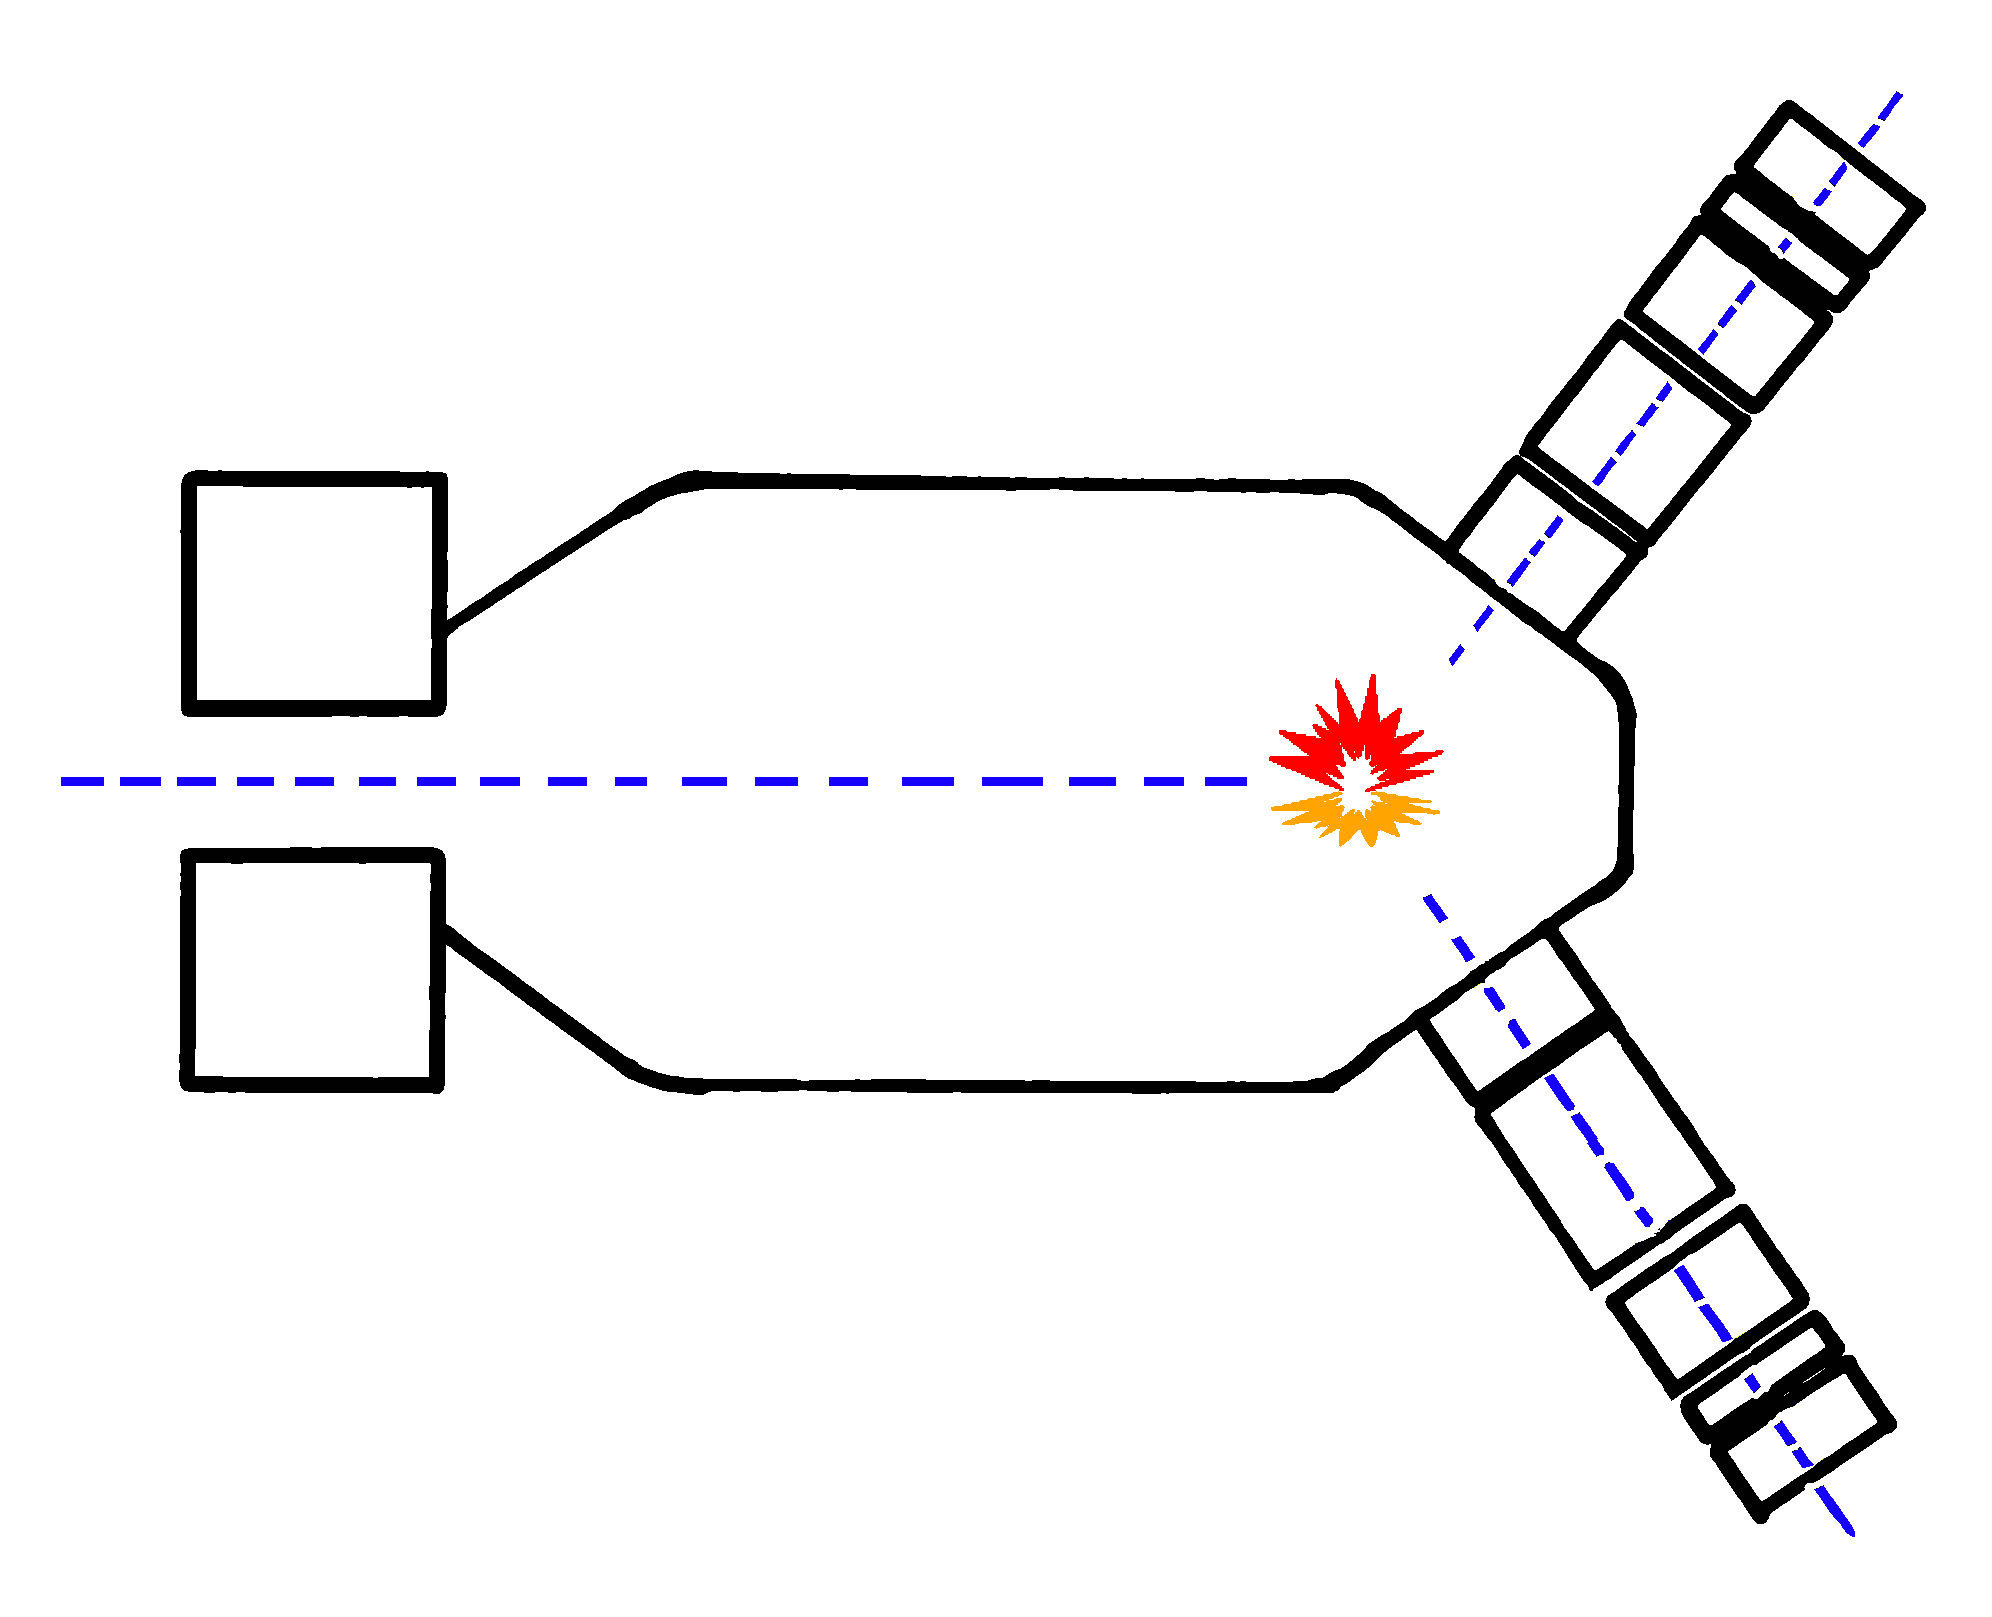
\includegraphics[scale=0.1]{figs/Christenson_apparatus.png}
\end{center}
\caption{\textit{Apparatus used in the Christenson et al experiment \cite{Christenson_apparatus_ref}}}
\label{Christenson_apparatus}
\end{figure}

\begin{figure}[h!]
\begin{center}
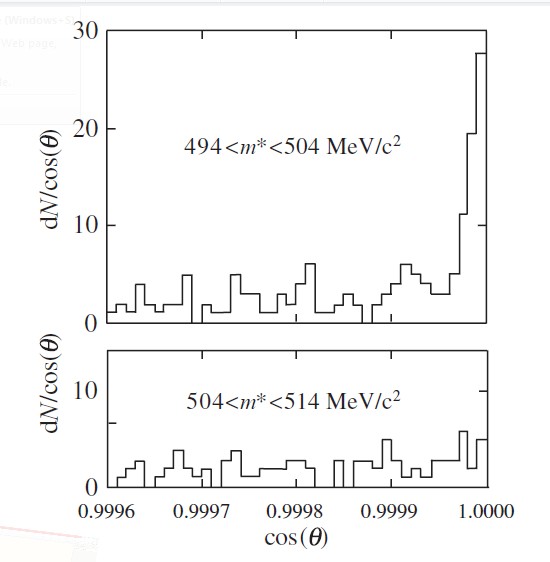
\includegraphics[scale=0.3]{figs/Christenson_results.png}
\end{center}
\caption{\textit{Results of the Christenson et al experiment \cite{FirstCPV}}}
\label{Christenson_results}
\end{figure}

The results of the Christensen et al experiment implies, that the weak eigenstates $\ket{K^{0}_{S}}$ and $\ket{K^{0}_{L}}$ are not aligned with the true $CP$ eigenstates $\ket{K^{0}_{1}}$ and $\ket{K^{0}_{2}}$. As in \cref{FirstKaonLinComb1} and \cref{FirstKaonLinComb2} one can write:

\begin{align}
\label{KaonLincomb11}
\ket{K^{0}_{S}} = a \ket{K^{0}_{1}} + b \ket{K^{0}_{2}} \\
\label{KaonLincomb12}
\ket{K^{0}_{L}} = a \ket{K^{0}_{1}} - b \ket{K^{0}_{2}}
\end{align}

\noindent Where $a$ and $b$ are complex numbers. The degree to which the states are not aligned is determined using the CP violation decay amplitudes and corresponding $CP$ conserving amplitudes \cite{Measurements_Direct_CPV_Kaons_KTev}: 

\begin{align*}
\eta_{+-} \vcentcolon= \frac{A(K^{0}_L \rightarrow \pi^+ \pi^-)}{A(K^{0}_S \rightarrow \pi^+ \pi^-)} = \epsilon + \epsilon' \\ 
\eta_{00} \vcentcolon= \frac{A(K^{0}_L \rightarrow \pi^0 \pi^0)}{A(K^{0}_S \rightarrow \pi^0 \pi^0)} = \epsilon - 2\epsilon' 
\end{align*}

\noindent The two complex parameters $\epsilon$ and $\epsilon'$ determine the amount of indirect and direct CPV, respectively. The indirect CPV is due to the $CP$ conserving decay of the $K^{0}_{1}(CP =1)$ component of the $K^{0}_{L}(CP=-1)$ to $CP=1$ final states, this is possible because of Kaon oscillations. The direct CPV is due to the $CP$ violating decay of the $K^{0}_{2}(CP =-1)$ component of the $K^{0}_{L}(CP=-1)$ to $CP=1$ final states, this is possible due to interference between different decay methods with the same final state, as in \cref{HEPP_intro_Perkins}.  

\begin{figure}[h!]
\begin{center}
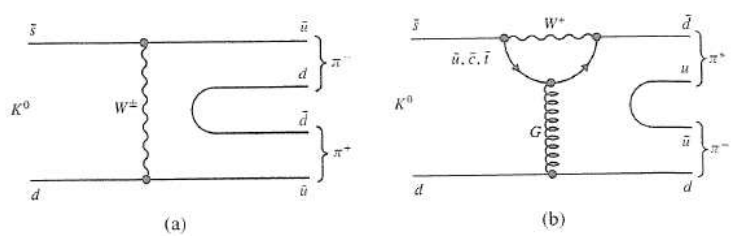
\includegraphics[scale=0.3]{figs/Perkins_Interference_Kaons.png}
\end{center}
\caption{\textit{Two possible decay modes for $K^{0} \rightarrow \pi^+ \pi^-$. (a) Tree diagram for decay by exchanging a W boson (b) Penguin diagram for decay via quark states \cite{HEPP_intro_Perkins}}}
\label{HEPP_intro_Perkins}
\end{figure}

\noindent However it is found that the direct CPV contribution is much smaller in this case. The indirect CPV almost completely dominates as can be seen from the similarity of the experimental values for $|\eta_{+-}|$ and $|\eta_{00}|$ \cite{PDGKaons}:

\begin{align*}
|\eta_{00}| = 0.002220 \pm 0.000011 &  & |\eta_{+-}| = 0.002232 \pm 0.000011 
\end{align*}  

\noindent If these values were significantly different it would suggest the amount of direct CPV would be comparable to the amount of indirect CPV, this of course is not the case. An experimentally determined value which illustrates this is the real part of the ratio of $\epsilon'$ to $\epsilon$ \cite{PDGKaons}:

\begin{equation*}
\mathbb{R} \bigg(\frac{\epsilon'}{\epsilon} \bigg)  = \bigg(1 - \bigg|\frac{\eta_{00}}{\eta{+-}}\bigg|\bigg) / 3 = 0.00166 \pm 0.00023
\end{equation*}

\smallskip

\noindent $|\epsilon|$ can also be determined using:

\begin{equation*} 
|\epsilon| = \big(2 |\eta_{+-}| + |\eta_{00}|\big)/3 = 0.002228 \pm 0.000011
\end{equation*} 

\smallskip

\noindent If the direct CPV contributions are ignored one can write \cref{KaonLincomb11} and \cref{KaonLincomb12} in terms of $\epsilon$:

\begin{align}
\label{KaonLincomb21}
\ket{K^{0}_{L}} = \frac{1}{(1+|\epsilon|^2)^{1/2}} \bigg[ \epsilon \ket{K^{0}_{1}} + \ket{K^{0}_{2}}\bigg] \\
\label{KaonLincomb22}
\ket{K^{0}_{S}} = \frac{1}{(1+|\epsilon|^2)^{1/2}} \bigg[ \ket{K^{0}_{1}} - \epsilon \ket{K^{0}_{2}}\bigg]
\end{align}

\smallskip

\noindent This linear combination shows the non-zero amplitude for weak eigenstate Kaons to oscillate between two different states with definite and opposite $CP$.

\subsection{Semileptonic decays}\label{Kevin:Kaon_semileptonic}

Decays of neutral Kaons to products containing leptons can be used to verify \cref{KaonLincomb21} and \cref{KaonLincomb22} as well as finding the asymmetry in the Kaon oscillation $K^{0} \leftrightarrow \bar{K}^{0}$. First the selection rules that play an important role in these decays must be discussed.

The $\Delta S = \Delta Q$ selection rule is an empirical rule backed up by some theoretical approximations. This rules states that in decays involving strangeness(S) and leptons, the change in the charge(Q) of the hadrons must be the same as the change in strangeness which must have a value of $\pm 1$. As an example consider semileptonic decays of the charged $\Sigma$ baryon. Two semileptonic decays of this baryon are:

\begin{align}
\label{Sigma1}
\Sigma^{-} (dds) \rightarrow n(udd) + e^{-} + \bar{\nu}_{e} \\
\label{Sigma2}
\Sigma^{+} (uus) \rightarrow n(udd) + e^{+} + \nu_{e}
\end{align}  

\noindent The feynmann diagram for decay \cref{Sigma1} can be drawn as in \cref{KevFeyn2}, while decay \cref{Sigma2} requires a diagram which must have at least two W bosons. It is clear that the diagram for $\Sigma^{-}$ is quite likely as it contains the Cabbibo favoured quark coupling $V_{ud}$ while any digram with two W bosons is unlikely, as for the $\Sigma^{+}$ decay. For this reason it is highly suppressed and has a braching ratio of $< (5\e{-6})$, which is consitent with it not existing in nature \cite{PDGKaons}. In comparrison the decay \cref{Sigma1} has a branching ratio of $(1.017 \pm 0.034) \e{-3}$. As there is no selection rule forbidding the second decay, the $\Delta S = \Delta Q$ rule was introduced to identify proceses like it. The change in strangeness and hadron charge for these decays can be found in \cref{DeltaSQruleTable}.

\begin{figure}[h!]
\begin{center}
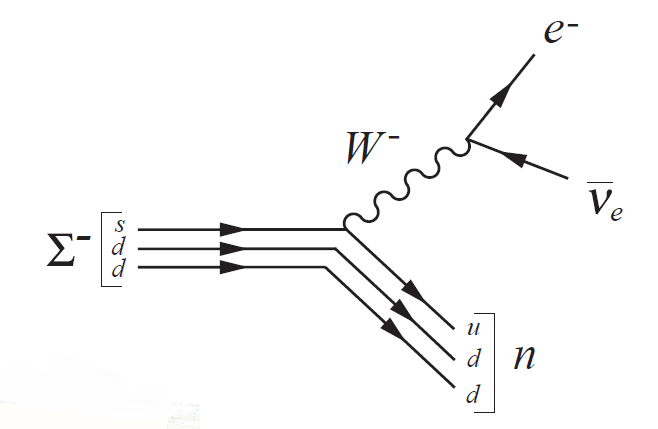
\includegraphics[scale=0.4]{figs/KevFeyn2.png}
\end{center}
\caption{\textit{Feynmann diagram for the $\Delta s = \Delta Q$ allowed decay of the $\Sigma^{-}$ boson to semileptonic final products}}
\label{KevFeyn2}
\end{figure}

\begin{table}[h!]
\caption{\textit{$\Delta S = \Delta Q$ selection rule table for the decays \cref{Sigma1} and \cref{Sigma2}}}
\centering
\setlength{\tabcolsep}{10pt}
\begin{tabular}{c| ccc}
\hline
Shown decay of   & $\Delta S$ & $\Delta Q$ & $\Delta S = \Delta Q$ \\ 
\hline \hline
$\Sigma^{-}$     &      +1    &    +1      & yes                   \\
$\Sigma^{+}$     &      +1    &    -1      & no                   \\
\hline
\end{tabular} 
\label{DeltaSQruleTable}
\end{table}

\smallskip

\noindent Where $\Delta A$ is the difference between the final and initial states of A such that $\Delta A = A_{final} - A_{initial}$. Also remember that the definition of strangeness assigns the strange quark a value of $-1$ and the anti-strange quark a value of $+1$. Thus it is clear that the decay \cref{Sigma2} violates the $\Delta S = \Delta Q$ selection rule. Similarly, a decay with $\Delta S = \pm 2$ will contain two W bosons and as a result will be very suppressed. In conclusion, $\Delta S = \Delta Q = \pm 1$ for an allowed process.      

This can now be applied to semileptonic decays of Kaons of the form $K \rightarrow \pi l \nu_{l}$. There are four Kaon decays that have this form:

\begin{align} %maybe put these decays directly into the table below, but may need t refer to them again
\label{Ksemi1}
K^{0} (d \bar{s}) \rightarrow \pi^{-} l^{+} \nu_{l} \\
\label{Ksemi2}
\bar{K}^{0} (s \bar{d}) \rightarrow \pi^{+} l^{-} \bar{\nu}_{l} \\
\label{Ksemi3}
K^{0} (d \bar{s}) \rightarrow \pi^{+} l^{-} \bar{\nu}_{l} \\
\label{Ksemi4}
\bar{K}^{0} (s \bar{d}) \rightarrow \pi^{-} l^{+} \nu_{l} 
\end{align} 

\smallskip

\noindent A similar table as before can now be constructed. See Table.(\ref{DeltaSQruleKsemi}), where the number shown refers to the equations above

\begin{table}[h!]
\caption{\textit{$\Delta S = \Delta Q$ selection rule table for the decays (\ref{Ksemi1}) - (\ref{Ksemi4})}}
\centering
\setlength{\tabcolsep}{10pt}
\begin{tabular}{c| ccc}
\hline
Shown decay of  & $\Delta S$ & $\Delta Q$ & $\Delta S = \Delta Q$ \\ 
\hline \hline
(\ref{Ksemi1})  &     -1     &     -1     & yes                   \\
(\ref{Ksemi2})  &     +1     &     +1     & yes                   \\
(\ref{Ksemi3})  &     -1     &     +1     & no                    \\
(\ref{Ksemi4})  &     +1     &     -1     & no                    \\
\hline
\end{tabular} 
\label{DeltaSQruleKsemi}
\end{table}

\noindent Thus it is clear that the only possible semileptonic decays of this form for $K^{0}$ and $\bar{K}^{0}$ are (\ref{Ksemi1}) and (\ref{Ksemi2}). As there is only one way for these processes to occur, there can be no interference between different processes and thus there can be no direct $CP$ violation in the semileptonic decays of Kaons \cite[pg. 10]{DAmbrosio}. So it is clear that the amplitudes of the $\Delta S = \Delta Q$ violating decays are:

\begin{equation*}
A(K^{0} \rightarrow \pi^{+} l^{-} \bar{\nu}_{l}) = A(\bar{K}^{0} \rightarrow \pi^{-} l^{+} \nu_{l}) = 0  
\end{equation*}

It is possible now to write these amplitudes in terms of $K^{0}_{S}$ and $K^{0}_{L}$. Using Eqn.(\ref{FirstKaonLinComb1}),(\ref{FirstKaonLinComb2}),(\ref{KaonLincomb21}) and (\ref{KaonLincomb22}) one finds\cite[pg. 11]{DAmbrosio}:

\begin{align*}
A({K}^{0}_{S} \rightarrow \pi^{+} l^{-} \bar{\nu}_{l}) = - A(K^{0}_{L} \rightarrow \pi^{+} l^{-} \bar{\nu}_{l}) = \frac{1 - \epsilon}{\sqrt{2}} A(\bar{K}^{0} \rightarrow \pi^{+} l^{-} \bar{\nu}_{l}) \\  
A({K}^{0}_{S} \rightarrow \pi^{-} l^{+} \nu_{l}) = A(K^{0}_{L} \rightarrow \pi^{-} l^{+} \nu_{l}) = \frac{1 + \epsilon}{\sqrt{2}} A(K^{0} \rightarrow \pi^{-} l^{+} \nu_{l})   
\end{align*}

\noindent Where terms of order $|\epsilon|^{2}$ have been neglected. The quantities $\delta_{L,S}$ can now be defined, which show the tendency for the oscillations $K^{0} \leftrightarrow \bar{K}^{0}$ to favour the matter particle state. Thus making a very small contribution to the matter anti-matter assymmetry.

\begin{equation*}
\delta_{L,S} = \frac{A({K}^{0}_{L,S} \rightarrow \pi^{-} l^{+} \nu_{l}) - A({K}^{0}_{L,S} \rightarrow \pi^{+} l^{-} \bar{\nu}_{l})}{A({K}^{0}_{L,S} \rightarrow \pi^{-} l^{+} \nu_{l}) + A({K}^{0}_{L,S} \rightarrow \pi^{+} l^{-} \bar{\nu}_{l})} \vcentcolon= 2 \mathbb{R}(\epsilon)
\end{equation*}

\noindent The experimental value for this quantity is $\delta_{L} = (3.27 \pm 0.12) \e{-3}$. Which clearly indicates a small tendency to favour the matter particle in oscillations. This can also be illustrated graphically by measuring the relative number(N) of $K^{0}$ and $\bar{K}^{0}$ particles over time in a beam consisting initially of $K^{0}$. See Fig.(\ref{AsymmetryPicFig})

\begin{figure}[h!]
\begin{center}
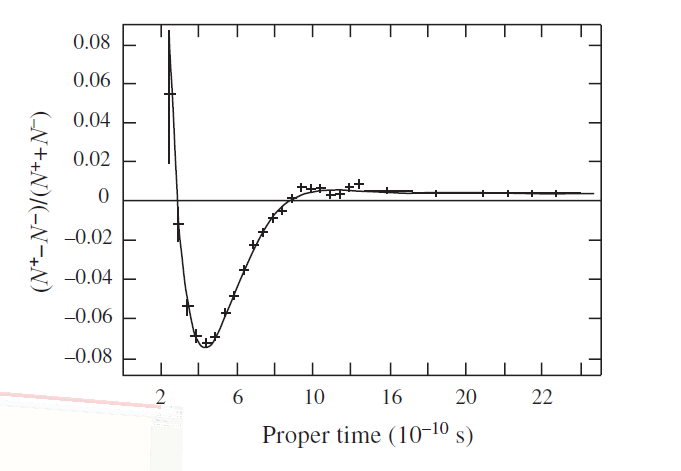
\includegraphics[scale=0.4]{figs/Asymmetry_pic}
\end{center}
\caption{\textit{Meaurements of observed Kaon semileptonic decays from a beam initially consisting of $K^{0}$ mesons which shows the oscillation between the states $K^{0}$ and $\bar{K}^{0}$ as well as the small asymmetry, favouring the matter particle \cite{AsymmetryPic}}}
\label{AsymmetryPicFig}
\end{figure}


\subsection{Testing $CPT$ conservation through Strangenss Oscillations}

The $CPT$ theorem links conservation of $CPT$ with Lorentz invariance. Thus to preserve the fundamental Lorentz symmetry physicists desperately hope $CPT$ is conserved. Here is presented some evidence that this is indeed the case. The theorem requires particles and their anti-particles to have the same masses and lifetimes. It has been stated previously that the $K^{0}_{L}$ and $K^{0}_{S}$ particles have very different lifetimes, but thankfully these are not a particle anti-particle pair. From earlier it is clear that $K^{0}$ and $\bar{K}^{0}$ are such a pair. Thus we aim to test $CPT$ conservation by measuring their mass difference.    

By investigating the time evolution of Kaon oscillations it is possible to measure their mass difference. By inverting the linear combinations in Eqn.(\ref{FirstKaonLinComb1}) and (\ref{FirstKaonLinComb2}) and neglecting the very small contribution of $\epsilon$, the flavour eigenstates are described by:

\begin{align*}
\ket{K^{0}(t)} = \frac{1}{\sqrt{2}} (\ket{K^{0}_{S}(t)} + \ket{K^{0}_{L}(t)}) \\
\ket{\bar{K}^{0}(t)}= \frac{1}{\sqrt{2}} (\ket{K^{0}_{S}(t)} - \ket{K^{0}_{L}(t)})
\end{align*} 

\noindent The time evolutions of the states are then written in terms of the mass and the lifetimes of the particles

\begin{align*}
\ket{K^{0}_{S}(t)} = \ket{K^{0}_{S}(0)} e^{-(im_{S}+\Gamma_{s}/2)t} \\
\ket{K^{0}_{L}(t)} = \ket{K^{0}_{L}(0)} e^{-(im_{L}+\Gamma_{L}/2)t} 
\end{align*} 

\noindent Where the exponential factor is as a result of the particle oscillations with time, and the fact that the particle will decay in time. We do the calculation for the $\bar{K}^{0}$ and simply state the result for the $K^{0}$. The probability amplitude(A) for the oscillations and then the probability of decay are determined using the linear combination:

\begin{align}
\ket{\bar{K}^{0}(t)} = \frac{1}{\sqrt{2}} & (\ket{K^{0}_{L}(0)} e^{-(im_{L}+\Gamma_{L}/2)t} - \ket{K^{0}_{S}(0)} e^{-(im_{S}+\Gamma_{s}/2)t}) \\
\bar{A} & = \frac{1}{2} (e^{-(im_{L}+\Gamma_{L}/2)t} - e^{-(im_{S}+\Gamma_{s}/2)t}) \\
\label{StrangenessOscillations1}
P(\bar{K}^{0}) = |\bar{A}|^{2} & = \frac{1}{4} \bigg[ e^{-\Gamma_{S}t} + e^{-\Gamma_{L}t} -2 e^{-(\Gamma_{S} + \Gamma_{L})t/2} \cos(t \Delta m )\bigg] \\
\end{align}

\noindent Where $\Delta m = |m_{S} - m_{L}|$. The extra factor of $1/{\sqrt{2}}$ comes from the initial condition that the experiment is started with a beam of $K^{0}$ particles which is equal parts $K^{0}_{L}$ and $K^{0}_{L}$. Thus $\ket{K^{0}_{L}(t=0)} = \ket{K^{0}_{S}(t=0)} = 1/{\sqrt{2}}$. The corresponding probability for $K^{0}$ is as follows:

\begin{equation}\label{StrangenessOscillations2}
P({K}^{0}) = |{A}|^{2} = \frac{1}{4} \bigg[ e^{-\Gamma_{S}t} + e^{-\Gamma_{L}t} + 2 e^{-(\Gamma_{S} + \Gamma_{L})t/2} \cos(t \Delta m )\bigg] \\
\end{equation}

For this experiment, the initial beam of Kaons is ``flavour tagged''. This is done by producing the $K^{0}$ particles in a strangeness conserving strong decay. The technique of tagging will be discussed further in section [JOHNS SECTION ON B]. The strangeness of the final state particles is then determined by looking for semileptonic decays discussed in section \ref{Kevin:Kaon_semileptonic}. The oscillations in time are made clear by plotting Eqn.(\ref{StrangenessOscillations1}) and (\ref{StrangenessOscillations2}) in Fig.(\ref{StrangenessOscillationsPic}). The decay rates for $K^{0}_{S}$ and $K^{0}_{L}$ are known so the results of this experiment can be used to determine $\Delta m$ for the weak eigenstate Kaons. This value is $\Delta m = (3.483 \pm 0.006) \e{-12}$.       

\begin{figure}[h!]
\begin{center}
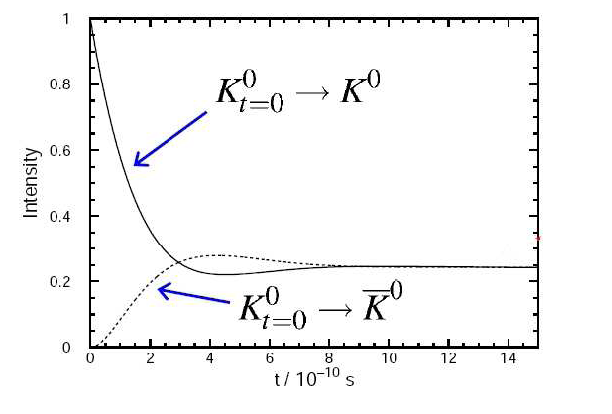
\includegraphics[scale=0.4]{figs/Strangeness_oscillations.png}
\end{center}
\caption{\textit{Theoretical predictions of the strangeness oscillations of a beam initially consisting of $K^{0}$ particles \cite{StrangenessPic}}}
\label{StrangenessOscillationsPic}
\end{figure}

To find ${\Delta m}_{flavour} = |m_{K^{0}} - m_{\bar{K}^{0}}|$ the link between $\Delta m$ above must be determined. The time dependent asymmetry in this system is given by:

\begin{equation*}
A_{CPT} = \frac{P[\bar{K}^{0} \rightarrow \bar{K}^{0}(t)] - P[{K}^{0} \rightarrow {K}^{0}(t)]}{P[\bar{K}^{0} \rightarrow \bar{K}^{0}(t)] + P[{K}^{0} \rightarrow {K}^{0}(t)]} = 4 \mathbb{R}({\delta})
\end{equation*}

\smallskip

\noindent Where $\delta$ is a $CPT$ violation parameter which can be written in terms of its projections parallel and perpendicular to the super weak direction $\phi_{SW} = \tan^{-1} (2 \Delta m / \Delta \Gamma)$ \cite{PDGKaons}:

\begin{align}
\label{CPTstrangeDelta1}
\delta_{\parallel} = \frac{1}{4} \frac{{\Delta \Gamma}_{flavour}}{\sqrt{\Delta m^{2} + \big(\frac{\Delta \Gamma}{2} \big)^{2}}} \\
\label{CPTstrangeDelta2}
\delta_{\perp} = \frac{1}{2} \frac{{\Delta m}_{flavour}}{\sqrt{\Delta m^{2} + \big(\frac{\Delta \Gamma}{2} \big)^{2}}}
\end{align}

Thus it is possible to determine $\mathbb{R}({\delta})$ in this experiment. Using other methods and other experiments $\mathbb{I}m({\delta})$ can be measured. So $\delta_{\parallel}$ and $\delta_{\perp}$ can be determined. Thus as shown in Eqn.(\ref{CPTstrangeDelta2}) $\Delta m_{flavour}$ can be determined. The current best result for this quantity is \cite{PDGKaons}: 

$$\frac{\Delta m_{flavour}}{m_{av}} < 6 \e{-19}$$ 

\noindent which is consitent with zero. Thus this experiment gives some confidence to $CPT$ conservation and the preservation of Lorentz invariance.      
  
  
  
  
